\section{Core Search Algorithm}
\sys applies a tree search to search through compositions of conditional assignments in the enumerated plan-space. In this section, we describe the core search algorithm and techniques to execute this algorithm efficiently.

{
\begin{algorithm}[t]
\KwData{Q, R, $\mathcal{P}$, $\gamma$, limit}

// Initialize priority queue of candidate programs\\
$S = \{NOOP\}$

\While{limit $> 0$}{
  \For{$s \in S$ }{
        
    Pop $s$ from the queue.
        
    \For{$p \in \mathcal{P}$}{
            $p' = p \circ s$ 
             
            $P.push(p', Q(p'(R)))$
        }
    
    
      $\bar{s} = \argmax_{s\in S} Q(s(R))$\\
      $S= \{s \in S\ |\ s < \gamma\times Q(\bar{s}(R)) \}$
    }
    
    limit -- //decrement limit
  }


\Return Highest priority item on the queue
\caption{Greedy Best-First Tree Search}
\label{alg:main}
\end{algorithm}
}

\subsection{Basic Algorithm}
Best-first search expands the most promising nodes chosen according to a specified cost function.
We consider a greedy version of this algorithm, which removes nodes on the frontier that are more than $\gamma$ times worse than the current best solution (\Cref{alg:main}).
Making $\gamma$ smaller makes the algorithm asympotically consistent but uses more memory to store the frontier, whereas $\gamma=1$ is a pure greedy search with minimal memory requirements.  

The frontier is modeled as a priority queue $S$ where the priority is the quality of the candidate program, and is initialized with a NOOP program with quality $Q(R)$.  
The algorithm iteratively extends all plans in the queue with a new conditional assignment from the set. 
Finally, let $\bar{s}$ be the highest quality plans in the queue.  The algorithm removes all programs whose quality is $<\gamma\times Q(\bar{s}(R))$ from the frontier.  
This process repeats until the candidate programs cannot be improved or an expansion limit is reached.
This process is progressive in the sense that the user can specify any expansion limit.

Since each plan $s' = s\circ p$ is the composition of a previous candidate program and a transformation, an obvious optimization is to materialize the output of $s(R)$ and compute $s'(R)$ as $T(s(R))$ over the materialized intermediate relation.
We leverage the fact that we can incrementally evaluate many quality functions of interest.
This means that we \emph{only have to materialize the delta}, which is the set of records modified by a particular conditional assignment.

\begin{figure}[t]
    \centering
    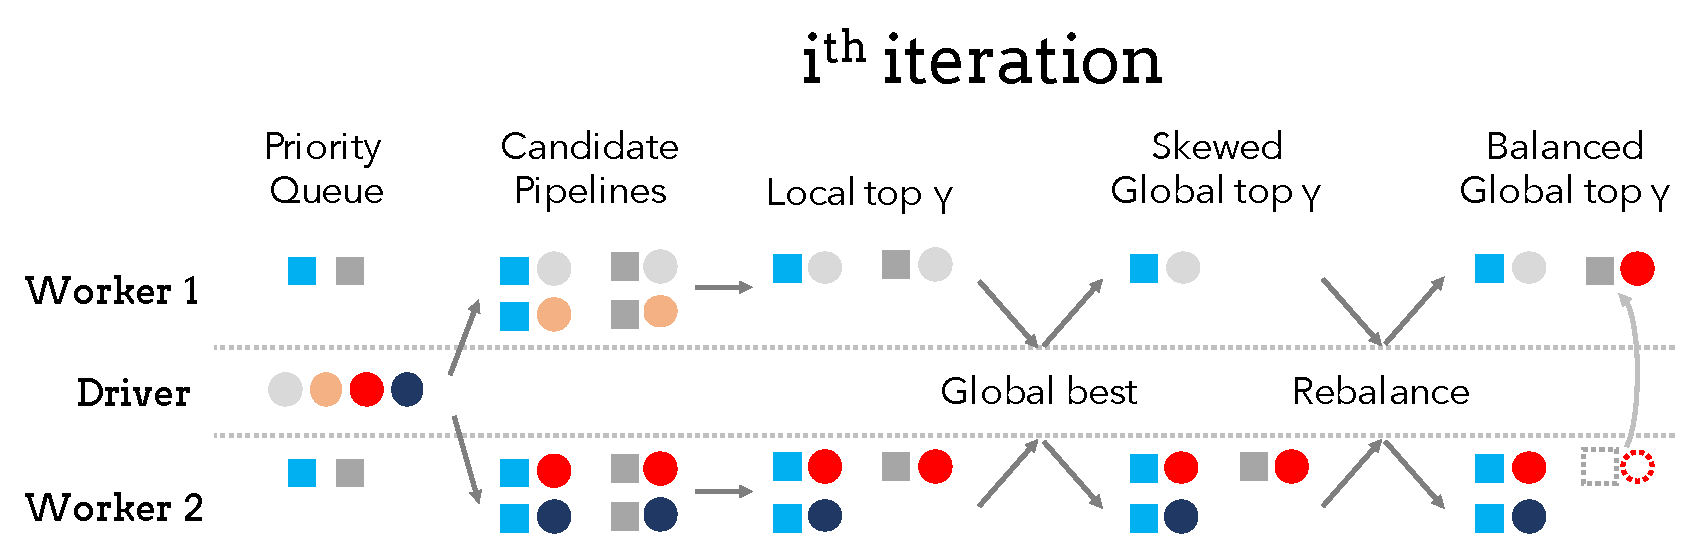
\includegraphics[width=\columnwidth]{figures/distributed.pdf}
    \caption{In each iteration, each worker starts with a subset of the priority queue (boxes).  The driver sends a subset of data transformations from $\Sigma$ (circles) to generate candidate programs (box-circles).  A series of synchronization points identify the globally top $\gamma$ candidates and redistributes them across the workers.   \label{fig:algo}}
\end{figure}

\subsection{Parallelization} 
Even with incremental evaluation, composing and evaluating $Q(s'(R))$ is the single most expensive operation in the search procedure.   
Plans can also be evaluated in a parallel fashion across multiple cores and multiple machines. 
The tree search algorithm distributes in a natural way.
Conceptually, we execute all expansions for a given plan $s$ in parallel.  We materialize the incremental changes in memory, and evaluate the quality of each $s' = p\circ s$ in parallel using a  thread pool.  Each thread drops a given $s'$ if its quality is lower than $\gamma\times$ the maximum quality from the previous \texttt{WHILE} iteration or the local thread.  At the end of the \texttt{WHILE} iteration, the threads synchronize to compute the highest quality, and flush the remaining candidates using the up-to-date quality value.

The implementation of this conceptual parallelization is a little bit more complex. 
Each worker is given a subset of candidate programs to locally evaluate and prune, and the main challenge is to reduce task skew through periodic rebalancing.  We use a worker-driver model with $j$ workers (\Cref{fig:algo}).

Let $S^{next} = S\times P$ be the set of candidate programs (e.g., 
\includegraphics[height=8pt]{figures/program.pdf}) to evaluate in the current iteration of the search algorithm. For instance, $S=\{NOOP\}$ in the first iteration, so the candidates are the set of individual data transformations $P$.   The driver assigns the input relation $R$ and $\frac{1}{j}$ of $P^{next}$ to each worker.  In the figure, the driver assigns a subset of $\Sigma$ to each worker.  Each worker evaluates and computes the top-$\gamma$ candidates based on the best worker-local quality.   The worker runs and caches the parents of its assigned candidate programs (
\includegraphics[height=8pt]{figures/sq-blue.pdf}, 
\includegraphics[height=8pt]{figures/sq-grey.pdf}) to incrementally compute the quality function.
  
Note that the worker-local top-$\gamma$ candidates are a superset of the top-$\gamma$ global candidates because the best local quality is $\le$ the global best.   Thus the workers synchronize with the driver to identify the global best candidate and further prune each worker's top candidates.  At this point, all candidate programs are within $\gamma$ of the globally best candidate, but their distribution across the workers can be highly skewed.  \sys performs a final rebalancing step, where each worker sends the number of un-pruned candidates to the driver.  Workers with more than $\frac{1}{j}$ of the total number redistribute the extras to workers with too few candidates.  When redistributing, workers communicate directly and do not involve the driver (e.g., Worker 2 sends 
\includegraphics[height=8pt]{figures/program-greyred.pdf} to Worker 1).   If the total number is $<k$, then candidates are randomly chosen to be replicated.  Only the programs and their qualities are sent; the program results are re-computed by the receiving worker.  This ensures that the priority queue in the next iteration is evenly distributed across all workers.
Our implementation uses Ray~\cite{ray} to schedule and parallelize the tasks.


\subsection{Collapsing Non-Interfering Paths}
As a heuristic, we also prune the search frontier by automatically combining plans that have disjoint predicates.
Every plan
